% First comes an example EPS file -- just ignore it and
% proceed on the \documentclass line
% your LaTeX will extract the file if required
% \begin{filecontents*}{example.eps}
% %!PS-Adobe-3.0 EPSF-3.0
% %%BoundingBox: 19 19 221 221
% %%CreationDate: Mon Sep 29 1997
% %%Creator: programmed by hand (JK)
% %%EndComments
% gsave
% newpath
%   20 20 moveto
%   20 220 lineto
%   220 220 lineto
%   220 20 lineto
% closepath
% 2 setlinewidth
% gsave
%   .4 setgray fill
% grestore
% stroke
% grestore
% \end{filecontents*}
%
\RequirePackage{fix-cm}
\RequirePackage{amsmath}     % included here an not with usepackage to prevent warning
%
%\documentclass{svjour3}                     % onecolumn (standard format)
\documentclass[smallcondensed]{svjour3}     % onecolumn (ditto)
% \documentclass[smallextended]{svjour3}       % onecolumn (second format) 
%\documentclass[twocolumn]{svjour3}          % twocolumn
%
\smartqed  % flush right qed marks, e.g. at end of proof
%
\usepackage{graphicx}
\usepackage{url}
\usepackage{algorithm}
\usepackage{algorithmic}
% \usepackage{amsmath}    % causes a warning about \vec redefinition with Springer class.
%
% \usepackage{mathptmx}      % use Times fonts if available on your TeX system
%
% insert here the call for the packages your document requires
%\usepackage{latexsym}
% etc.
%
% please place your own definitions here and don't use \def but
% \newcommand{}{}
%
% TODO
% Insert the name of "your journal" with
\journalname{Knowl Inf Syst}
%
\begin{document}

\title{Distributed ReliefF based Feature Selection in Spark
%\thanks{Grants or other notes about the article that should go on the front
%page should be placed here. General acknowledgments should be placed at the
%end of the article.}
}
% \subtitle{Do you have a subtitle?\\ If so, write it here}

%\titlerunning{Short form of title}        % if too long for running head

\author{Raul-Jose Palma-Mendoza \and
        Daniel Rodriguez \and
        Luis de-Marcos
}

% \author{First Author         \and
%         Second Author %etc.
% }


%\authorrunning{Short form of author list} % if too long for running head

\institute{ R. Palma \at
            Information Systems Engineering Department \\
            National Autonomous University of Honduras, Tegucigalpa, Honduras \\
              % Fax: +123-45-678910\\
              \email{raul.palma@unah.edu.hn}           %  \\
%             \emph{Present address:} of F. Author  %  if needed
            \and D. Rodriguez \and L. de-Marcos \at
            Computer Science Department, University of Alcal\'a \\
            Alcal\'a de Henares, 28871 Madrid            
}

\date{Received: date / Accepted: date}
% The correct dates will be entered by the editor


\maketitle

%% CHECK For most journals the figures should be 39 mm, 84 mm, 129 mm, or 174 mm wide and not higher than 234 mm.
%% CHECK Name your figure files with "Fig" and the figure number, e.g., Fig1.eps.

\begin{abstract}
Feature selection has become a key research area in the machine learning and data mining fields, by eliminating irrelevant and redundant features it has shown to be useful in reducing the effort required to process a dataset while maintaining or even improving the processing algorithm's accuracy. However, with the advent of big data, traditional algorithms designed for executing on a single machine lack scalability to deal with the increasing amount of data that is becoming available. ReliefF is one these traditional algorithms that has been successfully implemented in many feature selection applications. In this paper, we present a completely redesigned distributed version of the popular ReliefF algorithm. Our design is based in the novel Spark cluster computing model that has recently gained much attention due to its much faster processing times compared with Hadoop MapReduce model implementation. The effectiveness or our proposal is tested on four open datasets all of them with high number of instances, and two of them with also a high number of features. A traditional implementation is also tested on this datasets or portions of them. Results show that a traditional implementation is practically unable to handle such high amounts of data, and that our design can process them in a scalable way with much better time and memory consumption.


\keywords{First keyword \and Second keyword \and More}
% \PACS{PACS code1 \and PACS code2 \and more}
% \subclass{MSC code1 \and MSC code2 \and more}
\end{abstract}

\section{Introduction}
\label{intro}

In the last years we have witnessed a vast increase in the amount of data that is being stored and processed by organizations of all types. As stated in \cite{XindongWu2014}, the so-called big data revolution has come to us with many challenges but also with plenty of opportunities that these organizations are willing to take advantage of. According to \cite{Rajaraman2011}, the main challenge is to extract useful information or knowledge from these huge volumes of data, this data would enable us to predict or to better understand the phenomena involved in their generation. This tasks area tackled by the widely known fields: data mining and machine learning.

In addition, feature selection has grown over the last decade to establish as a crucial step in the reduction of dimensionality of these amounts of data \cite{Bolon-Canedo2015a}, by proving its usefulness to enhance the performance of many machine learning and data mining schemes. Feature selection algorithms are usually classified in any of three types: wrappers, filters and embedded methods. Wrappers refer to methods that require the learning of a classifier based on a single or on a subset of the original features, they are usually more computationally expensive. Filter methods rely only on the characteristics of data and are independent of any learning scheme, thereby requiring less computational effort. Finally, embedded methods refer to those techniques where the selection of features is done during the classification process. 

By the way, as mentioned by Garc\'ia et al. \cite{García2015}, another important feature selection classification is the one that comes from viewing the feature selection problem as a search problem, and thereby, classifies methods according to the types of search that is performed: exhaustive, heuristic and stochastic. However, not all feature selection techniques can be viewed as search problems, so a fourth category can be included: feature weighting.

In this context, ReliefF \cite{Kononenko1994} has become a widely applied feature weighting technique that estimates the quality of the features from a given dataset by assigning weights to each of them. It can be used as filter feature selection method by defining a significance threshold and selecting features with quality above it. Because of its advantages like: being able to work with nominal or continuous features, handling multi-class problems, detecting features interactions, handling missing data and noisy tolerance, it has been considered one of the most convenient filter-based feature selection methods available \cite{Bolón-Canedo2012}.

On the other hand, after its 2004 seminal paper Google's MapReduce \cite{Dean2004a,Dean2008} emerged as a programing model that simplified the development of scalable applications that process and generate large scale datasets. This applications are defined in terms of map an reduce tasks that are automatically parallelized by the framework and executed in clusters of thousands of machines, handling failures and scheduling resources. One important fact is that MapReduce was designed to run on commodity hardware, because it leads to lower costs per processor and per unit of memory of the cluster. The standard MapReduce implementation to date is Hadoop MapReduce \cite{hadoop}, an open source implementation mainly developed at Yahoo Labs. However, the framework uses disk writing between every MapReduce job with the object of failure recovering, but this becomes a bottleneck for iterative nature algorithms like the ones used in machine learning and data mining, including the original ReliefF algorithm. For that reason, Spark \cite{Zaharia2010} has gained much attention in the last couple of years, since it presents an improved model that is capable of handling most of its operations in-memory while maintaining the fault tolerance and scalability of MapReduce.

% TODO Recheck this paragraph after endind
In this paper we present a distributed and scalable redesign of the original ReliefF algorithm to the Spark computing model, enabling it to deal with much more bigger datasets in terms of instances and features than the traditional version would. In addition, after presenting and discussing the design of the algorithm we compare several runs of it with the traditional version implemented on the WEKA \cite{Hall2009} platform, using 4 open datasets with numbers of instances in the order of $10^6$ and a number of features that ranges in the order of $10^1$ until $10^3$. The main conclusion obtained is that is practically unfeasible to deal with such high amounts of data using the traditional version on standard hardware, while the distributed version is able to handle them smoothly.
% TODO
% Check previous The rest of this paper is organized as follows.
% Add fatMrMR citation!.
\section{Related Work}
\label{sec:relatedWork}
ReliefF was published by Kononenko in 1994 \cite{Kononenko1994} and since then, many applications, extensions and improvements have been published. Moreover, ReliefF itself is an extension of the original Relief algorithm developed by \cite{Kira1992}, the latter initially was limited to binary class problems while the former can handle multi-class problems. As a recent examples of those extensions, Reyes et al. \cite{Reyes2015} present three of them for multi-label problems and compares them with previous extensions for the same purpose. Zafra et al. \cite{Zafra2012} extend ReliefF to the problem of multi-instance learning. Greene et al. \cite{Greene2009} propose an adaptation to enhance ReliefF's ability to detect feature interactions called SURF (Spatially Uniform ReliefF) and use it in the genetic analysis of human diseases.

One of ReliefF's mayor flaws is its incapacity to detect redundant features, and hereby some attempts have been made to overcome this. For example, Li and He \cite{Li2016} use a forward selection algorithm to select non redundant critical quality characteristics of complex industrial products. Zhang et al. \cite{Zhang2008} combine ReliefF with the mRmR (minimal-redundancy-maximal-relevancy) algorithm \cite{Peng2005} to select non redundant gene subsets that best discriminate biological samples of different types. 

As it might be expected, most feature selection algorithms have asymptotic complexities that depend on the number of features and possibly in the number of instances, and in our case, ReliefF depends linearly on both \cite{Robnik2003}. Thereby, its performance gets compromised when faced with datasets with high dimensionality and/or high number of instances. For this reason, many attempts have been made to make feature selection, including ReliefF more scalable.

Recently, Canedo et al. in \cite{Bolon-Canedo2015}, propose a framework to deal with high dimensional data, distributing the dataset by features, processing in parallel the pieces, and then performing a merging procedure to obtain a single selection of features, however this method is oriented for high dimensional datasets and no tests were made with datasets with high amounts of instances. A some way similar approach is followed in Peralta et al. \cite{Peralta2015}, where the MapReduce model is used to implement a wrapper-based evolutionary search feature selection method. In this case, the data is split by instances, and on each of this pieces a evolutionary feature selection is performed. Furthermore, the reduce step basically uses a simple majority voting of the selected features with a user-defined threshold to define the definitive subset of features. Finally, tests were made with the Epsilon dataset, that we also use here (see section \ref{sec:experiments}).

Zhao et al. \cite{Zhao2012} presented a distributed parallel feature selection method based on variance preservation using the SAS High-Performance Analytics \footnote{\url{http://www.sas.com/en_us/software/high-performance-analytics.html}} proprietary software. Tests were made with both high dimensional and high number of instances datasets.

Kubica et al. \cite{Kubica2011}, develop parallel versions of three forward search based feature selection algorithms, a wrapper with a logistic regression classifier is used to guide the search that is parallelized using the MapReduce model.

It is also worth to mention the recent work of Wang et al. \cite{Wang2016}, that uses the Spark computing model to implement feature selection strategy for classification of network traffic. Their approach basically consists in two phases, first it generates a feature ranking based on the Fisher score, and then a forward search is done using a wrapper approach. Nevertheless, this has the clear disadvantage that can only be applied to continuous data.

As it can be seen, none of the above contributions implement a purely filter approach, even when the framework proposed in \cite{Bolon-Canedo2015} allows to apply filters on parts of the dataset, these results are then merged using a wrapper.

Finally, for the specific case of ReliefF, Huang et al. \cite{Huang2009} propose an optimization in order to improve the computation efficiency of ReliefF on large datasets, but this improvement is only useful when no instance random sampling step is performed for the weights approximation. In other words, it only works when the $m$ parameter (see section \ref{sec:reliefF}) is set equal to the number of instances. Furthermore, testing in their work is made with datasets with a number of instances in the order of $10^4$, that is still manageable by a single machine.

Summing up and to the best knowledge of the authors, no published contribution has ever attempted to redesign the ReliefF filter method to a distributed environment as is proposed here.

\section{ReliefF}
\label{sec:reliefF}

In this section, we provide a short discussion about the ReliefF algorithm published by Kononenko \cite{Kononenko1994} that will serve as a conceptual basis for the redesign presented in section \ref{sec:dreliefF}. As indicated earlier, ReliefF is based in the original Relief algorithm proposed by Kira and Rendell \cite{Kira1992}. They both share the same central idea, that consists in evaluating the quality of the features by their ability to distinguish the instances from one class to another in a local neighborhood, i.e. the best features are those contribute more to add distance between different class instances and contribute less to add distance between same class instances. ReliefF then, consists of an extension of the original Relief method thats is capable of working under multi-class, noisy and incomplete datasets.

% Use of mayus labels, ex: STATE, FOR is mandatory.
\begin{algorithm}
\caption{ReliefF~\cite{Robnik2003,Kononenko1994}}
\label{alg:reliefF}
\begin{algorithmic}[1]
% \STATE $Input: $ 
\STATE calculate prior probabilities $P(C)$ for all classes
\STATE set all weights $W[A] := 0.0$
\FOR{$i = 1$ \TO $m$}
  \STATE randomly select an instance $R_i$
  \STATE find $k$ nearest hits $H_j$
  \FORALL{classes $C \neq cl(R_i)$}
    \STATE from class $C$ find $k$ nearest misses $M_j(C)$
  \ENDFOR
  \FOR{$A := 1$ \TO $a$}
    \STATE $SH := - \sum_{j = 1}^{k} diff(A,R_i,H_j)$ \label{alg:diff1}
    \STATE $SM := \sum_{C \neq cl(R_i)} \left [ \left ( \frac{P(C)}{1 - P(cl(R_i))} \right )\sum_{j = 1}^{k} diff(A,R_i,M_j(C))  \right ]$ \label{alg:diff2}
    \STATE $W[A] := W[A] + (SH + SM) / (m \cdot k)$
    % \STATE $W[A]\!:=\!W[A]~-~\sum_{j = 1}^{k} diff(A,R_i,H_j) / (m \cdot k)
    %  + \sum_{C \neq class(R_i)} \left [ \left ( \frac{P(C)}{1 - P(class(R_i))} \right )\sum_{j = 1}^{k} diff(A,R_i,M_j(C))  \right ] / (m \cdot k)$
    % \STATE $W[A] := W[A] + \sum_{C \neq class(R_i)} \left [ \left ( \frac{P(C)}{1 - P(class(R_i))} \right )\sum_{j = 1}^{k} diff(A,R_i,M_j(C))  \right ] / (m \cdot k)$
  \ENDFOR
\ENDFOR
\end{algorithmic}
\end{algorithm}

Algorithm \ref{alg:reliefF} displays ReliefF's pseudo-code. As we can observe, it consists of a main loop that iterates $m$ times, where $m$ corresponds to the number of samples from data to perform the quality estimation. Each selected sample $R_i$ equally contributes to the $a$-size weights vector $W$, where $a$ is the number of features in the dataset. The contribution for the $A$-esim feature is calculated by first finding $k$ nearest neighbors of the actual instance for each class in the dataset. The $k$ neighbors that belong to the same class as the actual instance are called hits($H$), and the other $k \cdot (c - 1)$ neighbors are called misses ($M$), where $c$ is the total number of classes, an $cl(R_i)$, represents the class of the $i-$esim sample. Once neighbors are found, their respective contributions to $A$-esim feature, is calculated. The contribution of the hits collection is equal to the negative of the sum of the differences between the actual instance and each hit, observe that this is a negative contribution because only non desirable features should contribute to create differences between neighbor instances of the same class. Analogously, the contribution of the misses collection is equal to the weighted sum of the differences between the actual instance and each miss, this is of course a positive contribution because good features should help differentiate between instances of a different class. The weights for this summation is defined according to the prior probability of each class, calculated from the dataset. Finally, the sum of the contributions is divided by $k$ to calculate an average of them, and to maintain the definitive weights in the range $[-1, 1]$ a division by $m$ must be done. ReliefF's weights are interpreted in the positive direction: the higher the weight, the higher the corresponding feature's relevance.

% TODO initialization param for choosing the ramp or not.
Originally, the $diff$ function used to calculate the difference between two instances $I_1$ and $I_2$ for an specific feature $A$ was defined as shown on equation \ref{eq:diffNom} for nominal features, and as shown on equation \ref{eq:diffNumOrig} for numeric features. However, this latter one has been proved to cause an underestimation of numeric features with respect to nominal ones in datasets with both types of features. Thereby, a so-called ramp function, depicted in equation \ref{eq:diffNumRamp}, has been proposed in \cite{Hong1997} to deal with these problem. The basic idea of it, is to relax to equality comparison on equation \ref{eq:diffNumOrig} by using two thresholds: $t_{eq}$ is the maximum distance between two features to still consider them equal, and analogously, $t_{diff}$ is the minimum distance between two features to still consider them different. Their default values are set to $5\%$ and $10\%$ of the feature's value interval respectively. In our implementation, the use of the original $diff$ function or the ramp one for numeric features is selected through a initialization parameter. In addition, there are also versions of the $diff$ function that deal with incomplete data, however, since the datasets chosen for the experiments don't have missing values, we will not consider these versions in this work. Finally, the $diff$ function is used in two cases in the ReliefF algorithm, one in lines \ref{alg:diff1} and \ref{alg:diff2} for the calculation of the weight but also in the finding of the distances between the instances, defined as the sum of the differences over every feature (Manhattan distance).

\begin{equation}
\label{eq:diffNom}
diff(A,I_1,I_2) = \begin{cases}
0 & \text{if } value(A, I_1) = value(A, I_2),\\
1 & \text{otherwise }
\end{cases}
\end{equation}

\begin{equation}
\label{eq:diffNumOrig}
diff(A,I_1,I_2) = \frac{\left | value(A, I_1) - value(A, I_2) \right |}{ max(A) - min(A)}
\end{equation}

\begin{equation}
\label{eq:diffNumRamp}
diff(A,I_1,I_2) = \begin{cases}
0 & \text{if } d \leq t_{eq}, \\
1 & \text{if } d > t_{diff}, \\
\frac{d-t_{eq}}{t_{diff}-t_{eq}} & \text{if } t_eq < d \leq t_{diff}
\end{cases}
\end{equation}

\section{Spark Cluster Computing Model}

In this section, we discuss the main concepts behind the Spark computing model, focusing on those that will complete the conceptual basis for the description of our proposal in section \ref{sec:dreliefF}. We end up with a brief discussion about other existent computing models such as MapReduce, with the aim of justifying our selection of Spark. 

The main concept behind the Spark model is that of resilient distributed dataset or in short RDD. Zaharia et al. \cite{Zaharia2010,Zaharia2012} defined a RDD as a read-only collection of objects, that is partitioned and distributed across the nodes of a cluster, and has the ability to automatically recover lost partitions through the record of a lineage that knows where do the data came from and optionally, the calculations that went through it. What is more relevant, is that the operations run for an RDD are automatically parallelized by the Spark engine, this abstraction frees the programmer of having to deal with threads, locks and all the complexities involved in traditional parallel programming. 

There are two types of operations that can be executed on a RDD: actions and transformations. Actions are the mechanism that permit to obtain results from a Spark cluster, five commonly used actions are: $reduce$, $sum$, $aggregate$, $sample$ and $collect$. The action $reduce$ is used to aggregate the elements of a RDD, by applying a commutative and associative function that receives as arguments two elements of the RDD an returns one element of the same type. Action $sum$ is simply a shorthand for a reduce action that sums all the elements on the RDD. Next, action $aggregate$ has a similar behavior to $reduce$, but the return type can be different from type of the elements of the RDD, it works in two steps: the first one aggregates the elements of each partition and returns an aggregated value for each of them, the second one, merges these values between all partitions to a single one, that becomes the definitive result of the action. Lastly, actions $sample$ and $collect$ are also similar, the former takes an amount of elements and returns a random sample of this size from the RDD, and the latter, simply returns an array with all the elements in the RDD, this of course has to be done with care to prevent exceeding the maximum memory available at the driver.

On other hand, transformations are the mechanism for creating RDD from another. Since RDDs are read-only a transformation does not affect the original RDD but creates a new one. Maybe the three most important transformations are: $map$, $flatMap$ and $filter$. The first two: $map$ and $flatMap$ are similar, they return a new RDD that is the result of applying a function to each element of the original one. In the case of $map$, the function applied takes a single argument and returns a single element, thus the new RDD has the same number of elements that the original one. And in the case of $flatMap$, the applied function takes a single element but it can return zero or more elements, so the resulting RDD is not required to have the same number of elements than the original one. Finally, $filter$ is straightforward, it receives a boolean function to discriminate the dataset elements possibly returning a subset of it.

In what respects to the cluster's architecture, Spark follows the master-slave model, there is a cluster manager (master) through which, the so-called driver program can access the cluster, the driver coordinates the execution of a user application by assigning tasks to the executors, which are programs that run in the worker nodes (slaves), by default only one executor is run per worker. With regard to the data, the RDD partitions are distributed across the worker nodes, and the number of tasks launched by the driver on for each executor will be according to the number of partitions of the RDD residing in the worker. A detailed view of the discussed architecture with respect to the physical nodes can be seen on Figure \ref{fig:sparkArch}.

\begin{figure}
  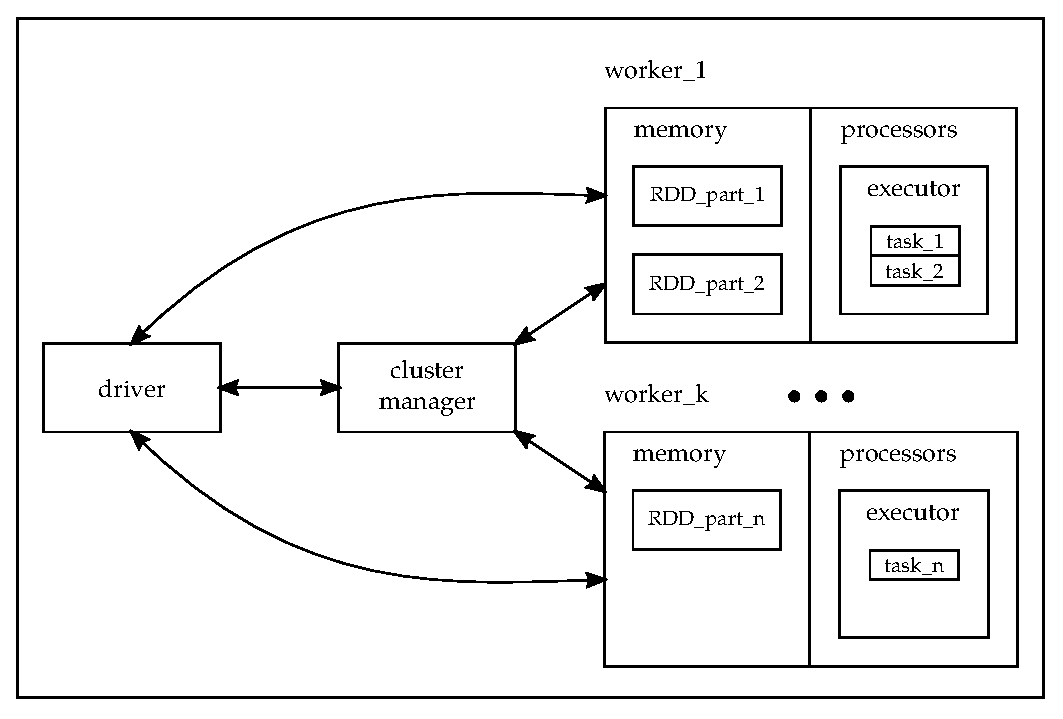
\includegraphics[width=1\textwidth]{figures/fig1.eps}
\caption{Spark Cluster Architecture}
\label{fig:sparkArch}
\end{figure}

\subsection{Other Cluster Computing Models}
Spark has quickly emerged between other cluster computing models that have already took much attention, being MapReduce the most relevant of them. This has happened due to the many advantages Spark has over them. First of all, Spark was designed from the beginning to efficiently handle iterative jobs in-memory, such as the ones used by many machine learning and data mining schemes. This has lead to the quick development of a machine learning library \cite{Meng2015} that contains Spark model redesigned algorithms such as the one in this work. Moreover, besides the Spark author's own comparison \cite{Zaharia2010,Zaharia2012}, others \cite{Shi2015} have shown that Spark is faster than MapReduce in most of the data analysis algorithms tested. Second, any MapReduce program can be directly translated to Spark, i.e. the MapReduce model can be completely expressed using the $flatMap$ and $groupByKey$ operations in Spark. And finally, from previous discussion is clear that Spark provides a wider range of operations other than $flatMap$ and $groupByKey$.

That said, its valuable to mention that other tools have already tried to fulfill the lack of efficient iterative job handling in MapReduce. Two of them are HaLoop \cite{Bu2010} and Twister \cite{Ekanayake2010}.  However, even when they have support for executing iterative MapReduce jobs, automatic data partitioning, and Twister has the ability to keep it in-memory, they lack  facility of loading a dataset in memory and then deciding what to with it, preventing an interactive data mining session over the data. Moreover, a recently published work \cite{Liu2016}, that included comparisons of parallelized versions of a neural network algorithm over Hadoop, HaLoop and Spark, concludes that Spark is the most efficient in all cases.

\section{Distributed ReliefF}
\label{sec:dreliefF}
In this section, we proceed to describe the proposed algorithm. The first design decision is where to concentrate the parallelization effort, ReliefF can be described as an embarrassingly parallel algorithm, since its outermost loop goes through completely independent iterations, each of these can be directly executed in different threads as stated by Robnik and Kononenko in ~\cite{Robnik2003}. However, parallelizing the algorithm in such way ties the parallelization to the number of samples $m$, and, as also stated by Robnik and Kononenko, this number of samples doesn't need to be very high when there is a high amount of data. In contrast, to achieve a good performance a high number of parallel tasks is needed. Thereby, a different approach must be followed. Continuing with Robnik and Kononenko discussion, ReliefF algorithm's complexity is $O(m \cdot n \cdot a)$, being $n$ the number of instances in the dataset and $m$ and $a$ the two already defined variables. Moreover, the most complex operation is the selection of the $k$ nearest neighbors, because first, the distance from the current sample to each of the instances must be calculated with $O(n \cdot a)$ steps, and then the selection must be done in $O(k \cdot log(n))$ steps. For this reasons, the parallelization is focused on these stages rather than on the independent iterations.

The first thing to note, is that ReliefF can be considered as a function applied to a dataset $DS$, to the number of samples $s$ and  to the number of neighbors $k$, that returns a $a-$size vector of weights $W$, as shown on equation \ref{eq:reliefFFunction}. Thus, ReliefF's algorithm can be interpreted as the calculation of each individual weight $W_A$, using equation \ref{eq:weightA}, where $sdiffs$ (equation \ref{eq:sumOfDiffs}) represents a function that returns the total sum of the differences in the $A-$esim feature between a given instance, and a set $NN_{C,i}$ of $k$ neighbors of the $i-$esim sample where all belong to the same given class $C$.

\begin{equation}
\label{eq:reliefFFunction}
relieff(DS,s,w) = W
\end{equation}

\begin{equation}
\label{eq:weightA}
W[A] = \sum_{i = 1}^{m} \left [ -sdiffs(A, R_i, cl(R_i)) + \sum_{C \neq cl(R_i)} \left [ \left ( \frac{P(C)}{1 - P(cl(R_i))} \right )
sdiffs(A,R_i,C) \right ] \right ]
\end{equation}

\begin{equation}
\label{eq:sumOfDiffs}
sdiffs(A,R_i,C) = \frac{1}{m \cdot k} \cdot \sum_{j = 1}^{k} diff(A,R_i,NN_{C,i,j})
\end{equation}

The dataset $DS$ can be defined (see equation \ref{eq:dataset}) as a set of $n$ instances each represented as a pair $I_i = (F_i,C_i)$ of a features vector $F_i$ and a class $C_i$. 
%TODO
% Need to define this? Moreover, equation $R$ is established as.

\begin{equation}
\label{eq:dataset}
DS = \left \{ (F_1,C_1),(F_2,C_2),\cdots,(F_n,C_n) \right \}
\end{equation}
  
Given the initial definitions, and assuming that the features types are stored as metadata, we start by calculating the maximum and minimum values for all continuous features in the dataset, these values will be needed by the $diff$ function (see equations \ref{eq:diffNumRamp} and \ref{eq:diffNumOrig}). This task, can be efficiently achieved by means of a $reduce$ action with a function $fmax$ ($fmin$) that given two instances returns a third one that contains the maximum (minimum) values for each continuous feature of both instances or anything if the feature is not continuous. This is shown for maximum values on equations \ref{eq:max}.

\begin{align}
\label{eq:max}
MAX & = DS.reduce(fmax) \nonumber \\
MAX & = (max(F_1[1],\cdots,F_n[1]), \cdots , max(F_1[a],\cdots,F_n[a]))
\end{align}

The next step consists in calculating the prior probabilities of all classes in $DS$, this is also a requirement of the $diff$ function. This values can be essentially obtained by means of a $map$ and a $reduceByKey$ transformations, the former simply returns a dataset with all instance classes paired with a value of one, and the latter sums this ones using the class as a key, thereby obtaining a set of pairs $(C_i, count(C_i))$, containing the classes and the number of instances in $DS$ belonging to that class, which can simply be divided by $n$ to obtain the priors. Equations \ref{eq:priors} depict the previous discussion, note that with the use of collect, $P$ is turned into a local collection rather than a RDD.

\begin{align}
\label{eq:priors}
f(I) & = (cl(I),1) \nonumber \\
g(a,b) & = a + b \nonumber \\
h((a,b)) & = (a, b / n) \nonumber \\
P & = DS.map(f).reduceByKey(g).map(h).collect() \nonumber \\
P & = \left \{ (C_1, prior(C_1)), \cdots , (C_c, prior(C_c)) \right \}
\end{align}

A rather short step, is the selection of the $m$ samples, this is accomplished with the use of the $takeSample$ action, as shown on equation \ref{eq:samples}.

\begin{equation}
\label{eq:samples}
R = \left \{ R_1,\cdots,R_m \right \} = DS.takeSample(m)
\end{equation}

Now we can proceed to the computationally intensive step of finding the $k$ nearest neighbors of each sample for each class. First, we find the distances from every sample $m$ to each of the $n$ instances. This can be directly accomplished by means of a $map$ transformation applied to $DS$ where for every instance $I$, a vector of distances from it to the $m$ samples is returned. Group of equations \ref{eq:distancesDataset}, depicts the previous discussion.

\begin{align}
\label{eq:distancesDataset}
distances(I) & = (distance(I,R_1), \cdots ,distance(I,R_m)) \nonumber \\
f(I) & = (I, distance(I)) \nonumber \\
DD & = DS.map(f) \nonumber \\
DD & = \left \{ (I_1, distances(I_1)),\cdots (I_n, distances(I_n))) \right \} 
\end{align}

Second and last, by using an $aggregate$ action we are able to obtain the nearest neighbors $NN$ matrix, where each element $NN_C,i$ is a vector with the $k$ nearest neighbors of a sample $R_i$ belonging to a class $C$. As said before, $aggregate$ action has two steps, the first step is defined in the function $localNN$, as its name suggests, this function returns a local neighbors matrix $LNN$ for each partition of the RDD, it has a similar structure as the $NN$ matrix but each vector element is treated as binary heap, where the $max$ value is the neighbor with the highest distance found, so while traversing the whole partition, whenever an instance with shorter distance than the $max$ is found, it is added to the heap, and if the heap is full the $max$ element is removed to make space. Thus, at the end the heap will contain the nearest neighbors in the local partition. One important thing to note here, is that each sample is effectively the nearest neighbor of the same class to itself, so a condition must be set to prevent including it in the $LNN$. The next step, is the merging of the local matrices, the defined function $mergeNN$ combines two local matrices by merging its individual binary heaps, keeping only the elements with shorter distances. Once both functions have been defined, a call to the $aggregate$ action can be performed, providing also an empty matrix $LNN$ structure (with empty heaps) so the $localNN$ can start aggregating neighbors to it. Lastly, it is worth to note that since the $NN$ is obtained via an action, it is a local object and not a RDD anymore and obtaining it concludes the complex step in the algorithm, step that has been fully parallelized. See equations \ref{eq:nearestNeighbors} for the above discussion.

% Last, by using a filter transformation over $DD$ and a $takeOrdered$ action we can find $NN_C,i$, a vector with the $k$ nearest neighbors of the class $C$ for a sample $R_i$, and repeat this process for all $m$ samples and all $c$ classes to obtain the $NN$ matrix (see equations \ref{eq:nearestNeighbors}), observing that since this matrix is obtained via an action, it is a local object and not a RDD anymore and obtaining it concludes the complex step in the algorithm, step that has been fully parallelized. Its also worth to note, that $takeOrdered$'s second argument defines how the ordering will be done, in our case, it will be based on the distance of every instance to the sample $R_i$, stored in the $i$-esim position of the distances vector inside every pair element of $DD$.

\begin{align}
\label{eq:nearestNeighbors}
NN & = \begin{bmatrix}
NN_{1,1} & \cdots  & NN_{1,m}\\ 
\vdots & \ddots  & \vdots \\ 
NN_{c,1} & \cdots & NN_{c,m} 
\end{bmatrix} \nonumber \\
NN_{C,i} & = (N_1,\cdots,N_k \mid \forall N \ cl(N) = C) \nonumber \\
localNN(I, LNN_{in}) & = LNN_{out}  \nonumber \\
mergeNN(LNN_a, LNN_b) & = LNN_{merged} \nonumber \\
NN & = DS.aggregate(emptyNN, localNN, mergeNN)
\end{align}

Once the $NN$ matrix is stored on the driver program, operations are not distributed in the cluster anymore, however, this is not a problem but a requirement, because $NN$ matrix is small: $c \times m$. The last remarkable step, consists in obtaining the matrix $SDIF$. Each element $SDIF_{C,i}$ represents an $a$-size vector, and each element of this vector stores the sum of the differences for the $A$-esim feature between the $NN_{c,i}$ group of neighbors and the $R_i$ sample. Moreover, each element the vector $SDIF_{C,i}$ can be calculated by mapping the $diff$ function over the $A$-esim feature of all the instances in the $NN_{C,i}$ vector and then summing this differences. Observe that this $map$ and $sum$ functions are not RDD-related anymore, but local equivalents that can be parallelized only on the driver's local threads. Finally, note that each element of each vector of the matrix $SDIF$ effectively represents the value shown on equation \ref{eq:sumOfDiffs}, thus, the final weights vector $W$, can be easily figured by applying the formula given on equation \ref{eq:weightA} using the already obtained $P$ set with the prior probabilities. Equations \ref{eq:sumOfDiffsMatrix} depict the above discussion and a resume of the algorithm's main pipeline discussed in this section is shown on Figure \ref{fig:relieffMain}.

\begin{align}
\label{eq:sumOfDiffsMatrix}
SDIF_{C,i} & = (sdiffs(1,R_i,C),\cdots,sdiffs(a,R_i,C)) \nonumber \\
f(N) & = diff(A,N,R_i) \nonumber \\
SDIF_{C,i,A} & = sdiffs(A,R_i,C) = NN_{C,i}.map(f).sum / (m \cdot k) \nonumber \\
SDIF & = \begin{bmatrix}
SDIF_{1,1} & \cdots  & SDIF_{1,m}\\ 
\vdots & \ddots  & \vdots \\ 
SDIF_{c,1} & \cdots & SDIF_{c,m} 
\end{bmatrix} \nonumber \\
\end{align}

% TODO A note about caching, after the testing has ended.

\begin{figure}
  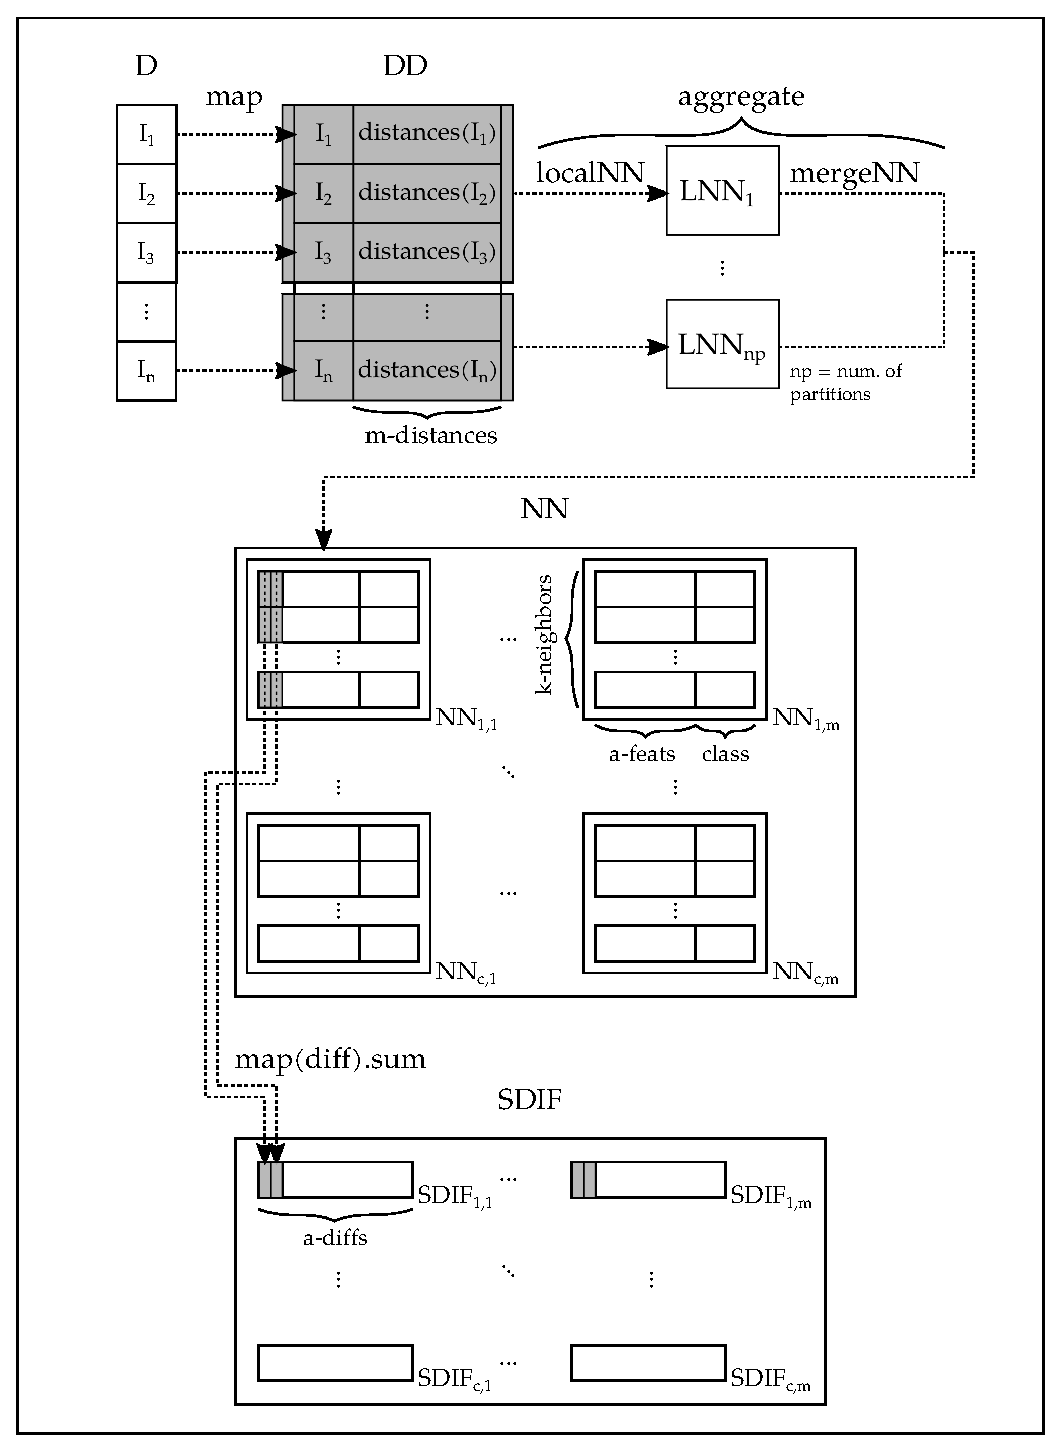
\includegraphics[width=1\textwidth]{figures/fig2.eps}
\caption{Distributed ReliefF Main Pipeline}
\label{fig:relieffMain}
\end{figure}

Before ending this section, there is one implementation issue that is worth to be mentioned. As previously said, a RDD is designed to be stored in memory, but this won't happen automatically, so if the RDD is going to be used in future operations it must be explicitly cached. In our case, after $DD$ is obtained, it should be cached, because it will be again be used to calculate the $NN$ matrix. Don't doing this will cause a serious performance downgrade because all the distances will need to be recalculated.

\section{Experimental Evaluation}
\label{sec:experiments}

In this section, empirical results obtained from different executions of the proposed algorithm are presented. The experiments where performed with the aim of testing the algorithm scalability, and its time and memory consumption with respect with the traditional version. 
%% TODO Include AUC testss?
For the realization of the tests, an 8-node cluster of virtual machines was used, one node is used as a master and the rest are slaves, the cluster runs over the following hardware-software configuration:

\begin{itemize}
\item Host Processors: 16 X Dual-Core AMD Opteron 8216.
\item Host Memory: 128 GB DDR2.
\item Host Storage: 7 TB SATA 2 Hard Disk.
\item Host Operating System: CentoOS 7.
\item Hypervisor: KVM (qemu-kvm 1.5.3).
\item Guests Processors: 2.
\item Guests Memory: 16 GB.
\item Guests Storage:  500 GB.
\item Java version: OpenJDK 1.8.
\item Spark version: 1.6.1.
\item HDFS version: 2.6.4.
\item WEKA version: 2.8.
\end{itemize}

For the first part of the tests, the ECBDL14 dataset was used, this dataset comes from the Protein Structure Prediction field, and it was recently used during the ECBLD14 Big Data Competition of the GECCO2014 international conference. The dataset has more approximately 33.6 million instances, 631 attributes, 2 classes, 98\% of negative examples and occupies about 56GB of disk space. All tests are run with a number of neighbors $k=10$, which is a typical choice \cite{Kononenko1994} and a relatively low number of samples $m=10$ because as shown by Robnik and Kononenko \cite{Robnik2003}, when a large amount of instances is available, lower values of $m$ are needed. In addition, HDFS is used to store all the datasets or samples of datasets in the experiments related to the distributed version. Conversely, the local file system is used for tests of the traditional version of ReliefF.

An important configuration issue refers to driver memory consumption. In Spark computation model, there is no communication between tasks, so all the tasks results will be sent to the driver, this is especially important for the $aggregate$ action, because every task performing the $localNN$ operation will return a $LNN$ matrix to the driver that then is going to be merged. The Spark configuration parameter $spark.driver.maxResultSize$ has a default value of 1 gigabyte but it was set to 4 for all the experiments performed. This is specifically important for tests involving higher matrix sizes: those with higher values of $m$ or $c$.

Figures {TODO}, show respectively the time and memory consumption behavior of the distributed version of ReliefF version versus the traditional one implemented in the WEKA\cite{Hall2009} platform for incrementally sized samples of the ECBDL14 dataset. For the comparison to be possible, the WEKA version was executed under the host environment, with no virtualization involved. The first thing to notice is that for the WEKA version a 30\% sample was the largest that could be tested, this is because using a 40\% sample would need more memory than the available in the system. This shows the lack of scalability of the traditional version. With respect to the distributed version, we observe that besides being able to handle the whole dataset, it preserves the linear behavior to number of instances the traditional version has, it is also able to process data in much less time, by leveraging the cluster nodes. 

Analogous results are obtained by varying the number of features and the number of samples as can be seen in figures {TODO.}, thereby confirming an empirical complexity equivalent to the original one: $O(m \cdot n \cdot a)$.

Another previously mentioned advantage of Spark that is designed to run in commodity hardware, by a simple look to the memory consumption of the traditional version, we infer that the required amounts of memory quickly grow beyond the limits of an ordinary computer. While in the distributed version, we observe that using nodes with 16GB of memory is enough to handle the task. Moreover, figures {TODO} show that even when the whole dataset does not fit in memory (after a 50\% sample and beyond), Spark is able to use a mixture of memory and disk storage to handle the task efficiently. 



Now, we delve into the topic of scalability. To keep times reasonable, the test was performed with 5\%, 10\% and 20\% samples of ECBDL14 dataset. Figures {TODO}, show the behavior of the distributed algorithm with respect to the number of cores used. As it can be seen, the first added cores greatly contribute the reduce the amount of time, but after a quantity $nc$ of introduced cores, the contribution is more subtle even reaching to be completely null. By observing the three figures, it is clear that the $nc$ quantity depends on the size of the dataset, so, larger datasets can take more benefit of larger amounts of cores. On the other hand, smaller datasets will face the case were they do not have enough partitions to be distributed over all the cluster nodes (figure 5\%), in this case, adding more nodes, will not cause any performance improvements.
Figures {5,10,y 20} also display with a dotted line the WEKA version behavior, since it can only take advantage of one core, the execution time is constant. However, the time is better than the distributed version in the case where one core is involved (TODO check this), clearly because, it doesn't have to deal with the driver scheduling, the selection of an executor and communication between both of them over the network, as the distributed version does.








% renice -15 -u qemu

% Testing schedule:
% Comprobar la teoría de que si el dataset no cabe en memoria es mejor no usar la cache R= FALSO, siempre es mejor almacenar en cache aunque sea una parte.
% La caché en disco no da mejoras, dado que el cálculo es relativamente simple, es mejor hacerlo otra vez, que escribir a disco.
% Comprobar si es mejor usar cache serializada o no, he visto que en cuestión de espacio no hay mucha diferencia pero en tiempo R= El espacio que ahorra ayuda a leer menos de disco y reducir el tiempo.
%Use https://github.com/jhclark/memusg/blob/master/memusg for memory tests, edited the followign line:
% 



We should note that this is quite typical behavior and usually we get stable estimates after 20-50 iterations, -> page 28 Theoretic

Check this:

% http://machinelearningmastery.com/an-introduction-to-feature-selection/

% The simple answer is that you should do feature selection on a different dataset than you train on (you're doing this already, so don't change this)---the effect of not doing this is you will overfit your training data. You must also not do feature selection on your test set, as this will inflate estimates of your models' performance (I think you already realise this as well, but I found it a little hard to understand the question precisely).

\section{Conclusions}



% \subsection{Subsection title}
% \label{sec:2}
% % as required. Don't forget to give each section
% % and subsection a unique label (see Sect.~\ref{sec:1}).
% \paragraph{Paragraph headings} Use paragraph headings as needed.

% % For one-column wide figures use
% \begin{figure}
% % Use the relevant command to insert your figure file.
% % For example, with the graphicx package use
%   \includegraphics{example.eps}
% % figure caption is below the figure
% \caption{Please write your figure caption here}
% \label{fig:1}       % Give a unique label
% \end{figure}
% %
% % For two-column wide figures use
% \begin{figure*}
% % Use the relevant command to insert your figure file.
% % For example, with the graphicx package use
%   \includegraphics[width=0.75\textwidth]{example.eps}
% % figure caption is below the figure
% \caption{Please write your figure caption here}
% \label{fig:2}       % Give a unique label
% \end{figure*}
% %
% % For tables use
% \begin{table}
% % table caption is above the table
% \caption{Please write your table caption here}
% \label{tab:1}       % Give a unique label
% % For LaTeX tables use
% \begin{tabular}{lll}
% \hline\noalign{\smallskip}
% first & second & third  \\
% \noalign{\smallskip}\hline\noalign{\smallskip}
% number & number & number \\
% number & number & number \\
% \noalign{\smallskip}\hline
% \end{tabular}
% \end{table}


%\begin{acknowledgements}
%If you'd like to thank anyone, place your comments here
%and remove the percent signs.
%\end{acknowledgements}

% BibTeX users please use one of
% \bibliographystyle{spbasic}      % basic style, author-year citations
\bibliographystyle{spmpsci}      % mathematics and physical sciences
%\bibliographystyle{spphys}       % APS-like style for physics
\bibliography{library}   % name your BibTeX data base

% Non-BibTeX users please use
% \begin{thebibliography}{}
% %
% % and use \bibitem to create references. Consult the Instructions
% % for authors for reference list style.
% %
% \bibitem{RefJ}
% % Format for Journal Reference
% Author, Article title, Journal, Volume, page numbers (year)
% % Format for books
% \bibitem{RefB}
% Author, Book title, page numbers. Publisher, place (year)
% % etc
% \end{thebibliography}

\end{document}
% end of file template.tex